\documentclass[handout]{beamer}
%==============================================================
% Common Beamer Preamble for Course Lectures: Training and Scaling Language Models
%==============================================================

\usepackage[utf8]{inputenc}
\usepackage[T1]{fontenc}
\usepackage{hyperref}
\usepackage{amsmath,amssymb,xcolor,multicol,booktabs,colortbl}
\usepackage{graphicx,listings}
\renewcommand{\figurename}{Figure.}
\renewcommand{\tablename}{Table.}

% ---- TikZ Libraries ----
\usepackage{tikz}
\usetikzlibrary{positioning,arrows.meta,shapes.geometric,calc,fit,backgrounds,decorations.pathreplacing}

% ---- Presentation defaults ----
\setbeamertemplate{navigation symbols}{}
\setbeamersize{text margin left=0.55cm,text margin right=0.55cm}
\setbeamerfont{title}{size=\LARGE,series=\bfseries}
\setbeamerfont{subtitle}{size=\large}

% ---- FontAwesome fallback ----
\IfFileExists{fontawesome5.sty}{%
  \usepackage{fontawesome5}%
}{%
  \providecommand{\faMicrochip}{}%
  \providecommand{\faComments}{}%
  \providecommand{\faTools}{}%
  \providecommand{\faCheckCircle}{}%
  \providecommand{\faExclamationTriangle}{}%
  \providecommand{\faImage}{}%
  \providecommand{\faRobot}{}%
  \providecommand{\faTerminal}{}%
  \providecommand{\faBook}{}%
  \providecommand{\faRedo}{}%
  \providecommand{\faLayerGroup}{}%
  \providecommand{\faCogs}{}%
  \providecommand{\faDatabase}{}%
  \providecommand{\faHdd}{}%
  \providecommand{\faNetworkWired}{}%
}

% ---- Theme Style and Semantic Colors ----
%==============================================================
% Centralized Semantic Color Definitions for LLMs Presentation
%==============================================================

% ---- Base Template / Theme Colors (Aligned with Palette B) ----
\definecolor{themenavy}{RGB}{22,70,102}       % Palette B primary cerulean: #164666
\definecolor{themeblue}{RGB}{22,70,102}       % Primary alias
\definecolor{primarylight}{RGB}{34,92,132}    % Primary light: #225c84
\definecolor{themeteal}{RGB}{0,159,176}       % Accent cyan-teal: #009fb0
\colorlet{main_color}{themenavy}
\colorlet{accent}{themeteal}

\definecolor{accentdark}{RGB}{0,108,120}      % Deep cyan-teal for contrast text
\definecolor{accentlight}{RGB}{56,178,214}    % Slate accent cyan: #38b2d6
\definecolor{leafred}{RGB}{197,93,61}         % Terracotta red for branches/leaves

% ---- Website Panel & Border Neutrals ----
\definecolor{panelbg}{RGB}{237,245,249}       % Course-panel: #edf5f9
\definecolor{panelborder}{RGB}{204,226,238}   % Course-border: #cce2ee

% ---- Code listing style (syntax highlights) ----
\definecolor{deepblue}{RGB}{22,70,102}
\definecolor{deepred}{rgb}{0.6,0,0}
\definecolor{deepgreen}{RGB}{0,135,150}
\definecolor{halfgray}{gray}{0.55}

% ---- Semantic Theme Navy / Cerulean Shades ----
\colorlet{themebluebg}{panelbg}               % Panel #edf5f9
\colorlet{themebluecard}{main_color!8}        % Mild card background fills
\colorlet{themeblueborder}{panelborder}       % Border #cce2ee
\colorlet{themebluemid}{themeteal!60}         % Accent mid-contrast
\colorlet{themebluedraw}{main_color!80}       % Strong outline draws/strokes

% ---- Semantic Secondary Accent Teal Shades ----
\colorlet{accentdarkbg}{themeteal!10}        % Light secondary background fills
\colorlet{accentdarkdraw}{themeteal}         % Secondary outlines/strokes/text/axes

% ---- Functional Colors: Success Green ----
\definecolor{successgreen}{RGB}{55,145,55}
\colorlet{successbg}{successgreen!8}
\colorlet{successdraw}{successgreen!75}

% ---- Functional Colors: Alert Red ----
\definecolor{alertred}{RGB}{197,55,55}
\colorlet{alertbg}{alertred!8}
\colorlet{alertdraw}{alertred!75}

% ---- Functional Colors: Warning Orange ----
\definecolor{warningorange}{RGB}{220,110,30}
\colorlet{warningbg}{warningorange!10}
\colorlet{warningdraw}{warningorange!80}

% ---- Terracotta Red Shades ----
\colorlet{leafredbg}{leafred!12}
\colorlet{leafreddraw}{leafred!80}

% ---- Accent Violet (SWE-bench / observe phases) ----
\definecolor{accentviolet}{RGB}{120,70,180}
\colorlet{accentvioletbg}{accentviolet!10}
\colorlet{accentvioletdraw}{accentviolet!80}

% ---- Post-Training Axis Blue ----
\definecolor{posttrainingblue}{RGB}{40,90,165}
\colorlet{posttrainingbg}{posttrainingblue!8}
\colorlet{posttrainingdraw}{posttrainingblue!75}

% ---- Harness Component Action Green ----
\definecolor{actiongreen}{RGB}{55,145,55}
\colorlet{actiongreenbg}{actiongreen!10}
\colorlet{actiongreendraw}{actiongreen!65}

% ---- Harness Component Persist Olive ----
\definecolor{persistolive}{RGB}{120,135,40}
\colorlet{persistolivebg}{persistolive!12}
\colorlet{persistolivedraw}{persistolive!70}

% ---- Harness Component Observe Violet ----
\colorlet{observevioletbg}{accentvioletbg}
\colorlet{observevioletdraw}{accentvioletdraw}

% ---- Neutrals (Grays/Blacks) ----
\colorlet{neutralbg}{black!4}             % Very light background fills
\colorlet{neutrallight}{black!30}         % Border frames/ticks/dividers
\colorlet{neutraldark}{black!75}          % Main body text/code listing text

% ---- Beamer Block Color Overrides (Premium Terracotta Theme) ----
\setbeamercolor{block title alert}{bg=leafreddraw,fg=white}
\setbeamercolor{block body alert}{bg=leafredbg}
\setbeamercolor{alerted text}{fg=leafreddraw}

\usepackage{../common/style}
\graphicspath{{../common/figs/}{figs/}}

% ---- Code Listing Config ----
\lstset{
  basicstyle=\ttfamily\footnotesize,
  keywordstyle=\bfseries\color{deepblue},
  emphstyle=\ttfamily\color{deepred},
  stringstyle=\color{deepgreen},
  commentstyle=\color{halfgray}\itshape,
  numbers=left, numberstyle=\tiny\color{halfgray},
  backgroundcolor=\color{codebg},
  frame=l, framerule=1.5pt, rulecolor=\color{themeteal},
  xleftmargin=10pt, framexleftmargin=4pt, numbersep=6pt,
  showstringspaces=false, breaklines=true,
  aboveskip=4pt, belowskip=4pt
}

% ---- Image Placeholder Utility ----
\newcommand{\slideimage}[2][3.8cm]{%
  \begin{center}
    \begin{tikzpicture}
      \node[draw=main_color, dashed, very thick, rounded corners,
        fill=themebluebg, minimum width=0.88\linewidth, minimum height=#1,
      text width=0.80\linewidth, align=center, font=\itshape, text=accentdark]
      {\textbf{[ FIGURE / DIAGRAM ]}\\[6pt] #2};
    \end{tikzpicture}
  \end{center}
}

% ---- Concept Highlight Card Utility ----
\newcommand{\conceptcard}[3]{%
  \begin{coursebox}{#1}{#2}#3\end{coursebox}%
}

% ---- Reusable teaching-slide components ----
\newcommand{\learninggoals}[4]{%
  \begin{frame}{What should be clear by the end?}
    \begin{enumerate}
        \setlength{\itemsep}{7pt}
      \item #1
      \item #2
      \item #3
      \item #4
    \end{enumerate}
  \end{frame}
}

\newcommand{\checkpoint}[2]{%
  \begin{frame}{Checkpoint: #1}
    \begin{block}{Think, then compare}
      #2
    \end{block}
  \end{frame}
}

\newcommand{\takeaways}[4]{%
  \begin{frame}{The durable ideas}
    \begin{enumerate}
        \setlength{\itemsep}{8pt}
      \item #1
      \item #2
      \item #3
      \item #4
    \end{enumerate}
  \end{frame}
}

\newcommand{\smallsource}[1]{%
  \vfill\hfill{\tiny\color{neutraldark}Source: #1}
}

% ---- Logo on content frames ----
\newif\ifplacelogo
\placelogotrue
\logo{\ifplacelogo
  \raisebox{-0.3ex}{
\includegraphics[height=0.4cm]{IMT_Atlantique_logo.png}}%
\fi}

\makeatletter
\define@key{beamerframe}{nologo}[true]{%
  \placelogofalse
}
\makeatother

% Fix Beamer bold font warning: substitute undefined T1/cmss/b/n with T1/cmss/bx/n
\DeclareFontShape{T1}{cmss}{b}{n}{<->ssub * cmss/bx/n}{}

% Default Author & Institute metadata
\author[Jonathan Lys]{Jonathan Lys}
\institute[IMT Atlantique]{IMT Atlantique}

% ---- Front Page / Title Slide Macro ----
% Displays Title + IMT Atlantique logo and Brain logo
\newcommand{\makelecturetitle}[1][Training and Scaling Language Models: From First Principles to Efficient Serving]{%
  \placelogofalse
  {
    \setbeamertemplate{footline}{}
    \settitletagline{#1}
    \settitlelogos{%
      \raisebox{-0.5\height}{
\includegraphics[height=1.15cm]{IMT_Atlantique_logo.png}}%
      \hspace{1.2em}%
      \raisebox{-0.5\height}{\includegraphics[height=1.15cm]{brain.pdf}}}
    \begin{frame}[plain]
      \titlepage
    \end{frame}
  }
  \placelogotrue
}

% Section TOC Frame
\AtBeginSection[]{\coursesectiondivider}

\title[TLM -- Session 12]{Session 12: Serving Systems\\[4pt]
\normalsize\itshape Scheduling Tokens under Latency and Memory Constraints}
\date{\today}

\begin{document}
\makelecturetitle
\begin{frame}{Lecture map}
  \tableofcontents
  \vfill
  \begin{block}{Guiding question}
    How does an inference engine turn irregular requests into efficient GPU work while protecting latency objectives?
  \end{block}
\end{frame}
\learninggoals
  {Trace a request through scheduler, cache manager, model runner, and output path.}
  {Explain continuous batching and chunked prefill at iteration granularity.}
  {Connect paged KV memory, admission control, and preemption.}
  {Design a serving benchmark with explicit workload and latency metrics.}

\section{From model forward to inference engine}

\begin{frame}{A serving engine coordinates four state machines}
  \begin{columns}[c]
    \begin{column}{0.52\linewidth}
      \begin{enumerate}
        \setlength{\itemsep}{7pt}
        \item request queue and admission policy
        \item iteration-level token scheduler
        \item KV-block allocator and prefix index
        \item model runner and sampled output stream
      \end{enumerate}
    \end{column}
    \begin{column}{0.44\linewidth}
      \begin{block}{One engine step}
        select tokens\\assign cache blocks\\execute model\\sample tokens\\update request state
      \end{block}
    \end{column}
  \end{columns}
  \smallsource{vLLM Anatomy and Hugging Face Continuous Batching}
\end{frame}

\begin{frame}{Prefill and decode compete for the same device}
  \begin{columns}[t]
    \begin{column}{0.47\linewidth}
      \begin{block}{Prefill request}
        many prompt tokens\\high parallelism\\large temporary attention work\\drives time to first token
      \end{block}
    \end{column}
    \begin{column}{0.47\linewidth}
      \begin{block}{Decode request}
        one token per active sequence\\growing KV reads\\latency sensitive\\drives inter-token latency
      \end{block}
    \end{column}
  \end{columns}
  \begin{alertblock}{Scheduling tension}
    A long prefill can increase throughput but block many decode tokens, causing visible latency spikes.
  \end{alertblock}
\end{frame}

\begin{frame}{Static batching waits for the slowest request}
  \begin{center}
  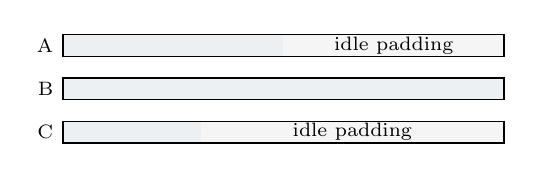
\begin{tikzpicture}[x=.7cm,y=.55cm,every node/.style={font=\scriptsize}]
    \foreach \y/\name in {3/A,2/B,1/C}{\node[left] at (0,\y+.25) {\name};}
    \fill[themebluecard] (0,3) rectangle (4,3.5);
    \fill[neutralbg] (4,3) rectangle (8,3.5);
    \fill[themebluecard] (0,2) rectangle (8,2.5);
    \fill[themebluecard] (0,1) rectangle (2.5,1.5);
    \fill[neutralbg] (2.5,1) rectangle (8,1.5);
    \draw (0,3) rectangle (8,3.5); \draw (0,2) rectangle (8,2.5); \draw (0,1) rectangle (8,1.5);
    \node at (6,3.25) {idle padding}; \node at (5.25,1.25) {idle padding};
  \end{tikzpicture}
  \end{center}
  \begin{alertblock}{Head-of-line effect}
    Completed sequences occupy batch slots until the longest member finishes. New work cannot enter even when capacity is available.
  \end{alertblock}
\end{frame}

\begin{frame}{Continuous batching repacks every iteration}
  \centering
  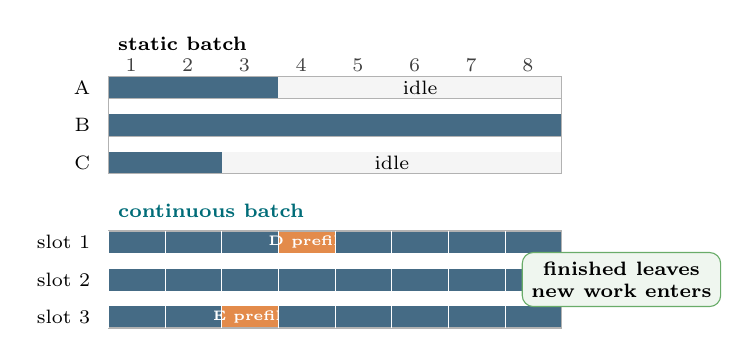
\begin{tikzpicture}[x=.72cm,y=.56cm,every node/.style={font=\scriptsize}]
    \node[anchor=west,font=\scriptsize\bfseries] at (2.2,6.65) {static batch};
    \node[anchor=west,font=\scriptsize\bfseries,text=accentdark] at (2.2,2.85) {continuous batch};
    \foreach \x in {0,...,7}{\node[text=neutraldark] at (2.6+\x,6.15) {\pgfmathparse{int(\x+1)}\pgfmathresult};}
    \foreach \y/\name in {5.4/A,4.55/B,3.7/C}{\node[left] at (2.05,\y+.25) {\name};}
    \foreach \x in {0,1,2}{\fill[themebluedraw] (2.2+\x,5.4) rectangle (3.2+\x,5.9);}
    \fill[neutralbg] (5.2,5.4) rectangle (10.2,5.9); \node at (7.7,5.65) {idle};
    \foreach \x in {0,...,7}{\fill[themebluedraw] (2.2+\x,4.55) rectangle (3.2+\x,5.05);}
    \foreach \x in {0,1}{\fill[themebluedraw] (2.2+\x,3.7) rectangle (3.2+\x,4.2);}
    \fill[neutralbg] (4.2,3.7) rectangle (10.2,4.2); \node at (7.2,3.95) {idle};
    \draw[neutrallight] (2.2,3.7) rectangle (10.2,5.9);
    \draw[neutrallight] (2.2,3.7)--(10.2,3.7); \draw[neutrallight] (2.2,4.55)--(10.2,4.55); \draw[neutrallight] (2.2,5.4)--(10.2,5.4);
    \foreach \y/\name in {1.9/slot 1,1.05/slot 2,.2/slot 3}{\node[left] at (2.05,\y+.25) {\name};}
    \foreach \x in {0,1,2}{\fill[themebluedraw] (2.2+\x,1.9) rectangle (3.2+\x,2.4);}
    \fill[warningdraw] (5.2,1.9) rectangle (6.2,2.4); \node[text=white,font=\tiny\bfseries] at (5.7,2.15) {D prefill};
    \foreach \x in {4,5,6,7}{\fill[themebluedraw] (2.2+\x,1.9) rectangle (3.2+\x,2.4);}
    \foreach \x in {0,...,7}{\fill[themebluedraw] (2.2+\x,1.05) rectangle (3.2+\x,1.55);}
    \foreach \x in {0,1}{\fill[themebluedraw] (2.2+\x,.2) rectangle (3.2+\x,.7);}
    \fill[warningdraw] (4.2,.2) rectangle (5.2,.7); \node[text=white,font=\tiny\bfseries] at (4.7,.45) {E prefill};
    \foreach \x in {3,4,5,6,7}{\fill[themebluedraw] (2.2+\x,.2) rectangle (3.2+\x,.7);}
    \draw[neutrallight] (2.2,.2) rectangle (10.2,2.4);
    \foreach \x in {0,...,7}{\draw[white] (2.2+\x,.2)--(2.2+\x,2.4);}
    \node[draw=successdraw,fill=successbg,rounded corners,align=center,font=\scriptsize\bfseries] at (11.25,1.3) {finished leaves\\new work enters};
  \end{tikzpicture}
  \vspace{3pt}
  \begin{block}{Scheduling unit}
    Repack useful decode tokens and prefill chunks every step, subject to token and KV-block budgets.
  \end{block}
\end{frame}

\section{Token and memory scheduling}

\begin{frame}{A token budget bounds work per engine step}
  Suppose the iteration budget is $N_{\max}$ scheduled tokens.
  \[
    N_{\text{decode}}+N_{\text{prefill}}\le N_{\max}
  \]
  \begin{itemize}
    \setlength{\itemsep}{8pt}
    \item Every active decode sequence usually asks for one token.
    \item Remaining capacity can admit prompt tokens.
    \item Cache-block availability may be the tighter constraint.
  \end{itemize}
  \begin{alertblock}{Policy matters}
    Prioritizing decode protects inter-token latency. Prioritizing large prefills may improve throughput but delay active users.
  \end{alertblock}
\end{frame}

\begin{frame}{Chunked prefill turns long prompts into schedulable pieces}
  Instead of scheduling a 16k-token prompt atomically, split it into chunks that share iterations with decode work.
  \begin{columns}[t]
    \begin{column}{0.47\linewidth}
      \begin{block}{Benefits}
        lower head-of-line blocking\\bounded iteration size\\better prefill-decode mixing
      \end{block}
    \end{column}
    \begin{column}{0.47\linewidth}
      \begin{alertblock}{Costs}
        more scheduling boundaries\\possible loss of prefill efficiency\\partial-request state
      \end{alertblock}
    \end{column}
  \end{columns}
  Chunk size is a latency-throughput knob, not a universal constant.
\end{frame}

\begin{frame}{Paged KV allocation matches irregular lifetimes}
  \begin{itemize}
    \setlength{\itemsep}{7pt}
    \item Divide KV memory into fixed-size physical blocks.
    \item Map each request's logical token blocks to any free physical blocks.
    \item Allocate as the sequence grows and return blocks on completion.
    \item Share immutable prefix blocks when requests have identical prefixes.
  \end{itemize}
  \begin{block}{What paging solves}
    External fragmentation and maximum-length over-reservation are reduced because requests need not occupy one contiguous region.
  \end{block}
  \begin{alertblock}{What remains}
    Internal slack in the last block, allocator metadata, capacity limits, and bandwidth cost of reading the cache.
  \end{alertblock}
\end{frame}

\begin{frame}{Prefix caching trades index work for avoided prefill}
  A cache hit can reuse KV blocks for an identical token prefix.
  \begin{columns}[t]
    \begin{column}{0.47\linewidth}
      \begin{block}{Works well for}
        repeated system prompts\\shared document prefixes\\branching completions
      \end{block}
    \end{column}
    \begin{column}{0.47\linewidth}
      \begin{alertblock}{Correctness conditions}
        identical model and adapter\\identical token IDs and positions\\compatible cache precision and layout
      \end{alertblock}
    \end{column}
  \end{columns}
  Measure hit rate, tokens avoided, retained-block cost, and eviction behavior together.
\end{frame}

\begin{frame}{Admission control prevents memory collapse}
  Before admitting work, estimate required blocks from prompt length, current cache, and maximum generation policy.
  \begin{itemize}
    \setlength{\itemsep}{7pt}
    \item queue when safe cache capacity is unavailable
    \item reject or cap requests outside the service contract
    \item preempt lower-priority work only under a declared policy
    \item distinguish recomputation preemption from host-memory swapping
  \end{itemize}
  \begin{alertblock}{Overcommit is not free}
    Preemption can recover capacity but adds wasted compute, extra latency, and tail-risk amplification.
  \end{alertblock}
\end{frame}

\begin{frame}{CUDA graphs reward stable execution shapes}
  Capturing a repeated GPU execution removes CPU launch overhead, but dynamic batches change shapes and memory addresses.
  \begin{columns}[t]
    \begin{column}{0.47\linewidth}
      \begin{block}{Engine strategy}
        capture a set of padded batch shapes\\reuse stable buffers\\fall back for unsupported shapes
      \end{block}
    \end{column}
    \begin{column}{0.47\linewidth}
      \begin{alertblock}{Trade-off}
        More capture sizes reduce padding but consume memory and operational complexity.
      \end{alertblock}
    \end{column}
  \end{columns}
\end{frame}

\checkpoint{schedule by hand}
  {An iteration budget is 16 tokens. Ten sequences need decode, one waiting prompt has length 20, and cache capacity is available. Propose the next two iterations under a decode-first chunked-prefill policy.}

\section{Measure the service, not a toy loop}

\begin{frame}{Latency is a distribution with several clocks}
  \small
  \begin{tabular}{@{}>{\raggedright\arraybackslash}p{.20\linewidth}>{\raggedright\arraybackslash}p{.35\linewidth}>{\raggedright\arraybackslash}p{.35\linewidth}@{}}
    \toprule
    Metric & Definition & Dominant factors \\
    \midrule
    queue time & arrival to admission & load and policy \\
    TTFT & arrival to first token & queue plus prefill \\
    inter-token latency & time between output tokens & decode schedule and batch \\
    end-to-end latency & arrival to completion & all phases and output length \\
    throughput & completed or output tokens per second & batching and saturation \\
    \bottomrule
  \end{tabular}
  \vfill
  Report median and tail percentiles. A good average can hide an unusable p99.
\end{frame}

\begin{frame}{Open-loop and closed-loop loads answer different questions}
  \begin{columns}[t]
    \begin{column}{0.47\linewidth}
      \begin{block}{Closed loop}
        Each client waits for completion before sending again. Offered load falls automatically when the server slows.
      \end{block}
    \end{column}
    \begin{column}{0.47\linewidth}
      \begin{block}{Open loop}
        Arrivals follow an external process. Queues grow when demand exceeds capacity, revealing overload behavior.
      \end{block}
    \end{column}
  \end{columns}
  \begin{alertblock}{Benchmark declaration}
    Report arrival process, prompt and output distributions, sampling settings, concurrency, warmup, and duration.
  \end{alertblock}
\end{frame}

\begin{frame}{A useful benchmark sweeps the operating curve}
  \begin{enumerate}
    \setlength{\itemsep}{7pt}
    \item choose a representative request-length distribution
    \item increase arrival rate or concurrency gradually
    \item record TTFT, inter-token latency, throughput, cache occupancy, and preemptions
    \item identify the saturation knee and tail-latency cliff
    \item compare policies at matched service-level objectives
  \end{enumerate}
  \begin{block}{The right conclusion}
    ``Policy A delivers more tokens/s while keeping p99 TTFT below the declared threshold for workload W.''
  \end{block}
\end{frame}

\begin{frame}{Read metrics as one coupled system}
  \begin{itemize}
    \setlength{\itemsep}{7pt}
    \item rising queue time with stable GPU time means admission is saturated
    \item TTFT spikes with stable decode latency suggest long prefills or queueing
    \item growing preemptions suggest cache overcommit
    \item high cache occupancy with low throughput suggests bandwidth or scheduler inefficiency
    \item lower mean latency with worse p99 may indicate unfair prioritization
  \end{itemize}
\end{frame}

\checkpoint{serving report}
  {Define a workload, one service-level objective, the policy under test, a baseline, and the five measurements needed to explain both throughput and tail latency.}

\takeaways
  {An inference engine schedules token work and cache state at every iteration.}
  {Continuous batching removes static slots, while chunked prefill controls head-of-line blocking.}
  {Paged memory, prefix reuse, admission, and preemption jointly determine capacity.}
  {Serving claims require representative arrivals plus throughput and tail-latency evidence.}
\end{document}
